\chapter{Peer to Peer}
Nel paradigma P2P tutti gli host agiscono sia da client che da server.
Tutti i nodi possono avere la stessa importanza all'interno della rete e si possono aggiungere / rimuovere nodi in ogni momento.
E' possible anche avere alcuni nodi piu' potenti e/o con funzionalità diverse rispetto ai nodi \textit{semplici}, i supernodi.
\section{Implementazioni}
Come e' possibile pero' tener traccia di tutti i nodi della rete (e i loro contenuti)?
\subsection{Directory centralizzata}
In questa implementazione si ha un server centrale che mantiene un registro di chi entra ed esce dalla rete, oltre alle loro informazioni.
Perciò un nuovo nodo che entra nella rete comunica con il server centrale per \textit{registrarsi} e ricevere le rotte verso gli altri.
Se il server non e' raggiungibile, \redtext{l'intera rete crolla}.
\subsection{Reti decentralizzate non strutturate}
In questo caso i dati sono ripartiti tra tutti i nodi senza una precisa configurazione. Cio porta a difficoltà nel localizzare le risorse ma l'aggiunta e la rimozione di nodi e' un'operazione molto semplice.
Se un nodo riceve una Query e possiede il file richiesto risponde con QueryHit in reverse path, altrimenti inoltra la richiesta ai suoi vicini.
Questo approccio porta a \redtext{flooding} della rete dato che ogni richiesta e' una nuova connessione da aprire.

Un approccio che combina i due appena descritti e' la \bluetext{copertura gerarchica}.
In questo caso ogni peer puo': essere un \bluetext{group leader} se potente in banda o risorse, oppure un nodo \bluetext{semplice} e viene assegnato ad un group leader.
Si hanno quindi connessioni \textit{peer $\leftrightarrow$ GL} e tra alcune coppie \textit{GL $\leftrightarrow$ GL}.
Il GL tiene traccia del contenuto dei figli associando gli hash dei file con gli indirizzi IP dei peer che possono trasmetterlo.
\subsection{Reti decentralizzate strutturate}
Nelle reti strutturate il posizionamento delle risorse segue dei principi molto rigidi. L'aggiunta e la rimozione di nodi dalla rete e' un'operazione costosa.

Vedi reti strutturate DHT.

\chapter{Sicurezza}
\section{Chiave Simmetrica}
Si utilizza la stessa chiave per cifrare e decifrare il messaggio.
Richiede un canale sicuro per lo scambio della chiave.
\section{Chiave Asimmetrica}
Ognuno possiede due chiavi, una pubblica e una privata.
La chiave pubblica serve a cifrare un messaggio che puo' essere decifrato soltanto dalla chiave privata associata.
Chi vuole ricevere un messaggio deve spedire la sua chiave pubblica al mittente.
\section{Message digest}
Ci sono casi in cui non e' necessario che un messaggio resti segreto, ma c'e' bisogno di verificarne l'integrità. Si utilizzano funzioni hash per produrre un digest di lunghezza fissa a partire da un messaggio qualunque.
\section{Message Authentication Code}
\section{Firma digitale}
\section{IPSec}
E' un insieme di protocolli per fornire sicurezza a livello di rete.
Si puo' applicare in due modalità.
\subsection{Modalità trasporto}
Protegge i dati passati dal livello di trasporto al livello di rete.
\begin{center}
    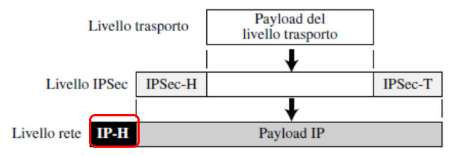
\includegraphics[width=0.9\textwidth]{ipsec-tr}
\end{center}
\redtext{L'header IP non e' protetto}
\subsection{Modalità tunnel}
In questo caso l'intero datagramma IP e' incapsulato all'interno di un nuovo livello IPSec, a sua volta inserito dentro un nuovo livello di rete.
\begin{center}
    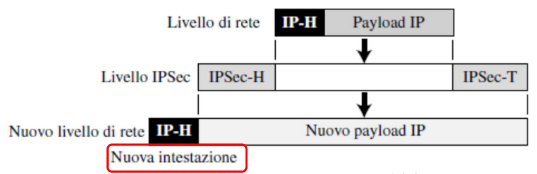
\includegraphics[width=0.9\textwidth]{ipsec-tu}
\end{center}
\subsection{Encapsulating Security Payload}
